\section{Polarimetría}
\subsection{Polarización}
\begin{frame}{\secname : \subsecname}
  \begin{figure}
    \centering
    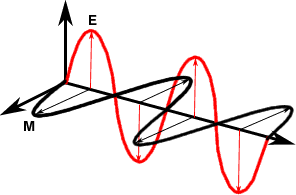
\includegraphics[scale=0.5]{fig:onda.png}
    \caption{Una onda electromagnética está caracterizada además de por la fase y la potencia por el plano de polarización.}
    \label{}
  \end{figure}
\end{frame}
%--- Next Frame ---%

\begin{frame}{\secname : \subsecname}
  \begin{figure}
    \centering
    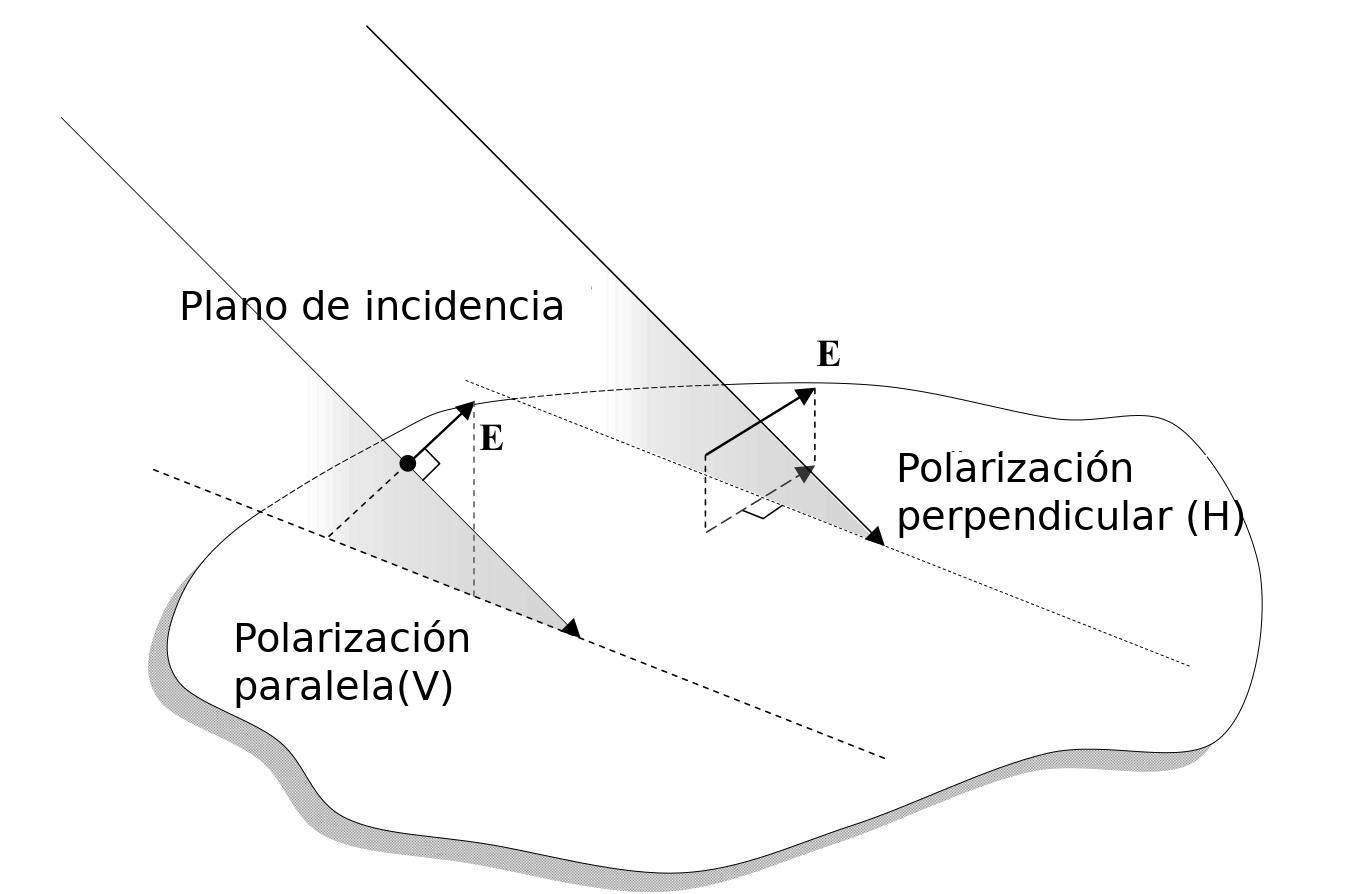
\includegraphics[width=0.6\textwidth]{fig:polarizacion.png}
    \caption{Algunos SAR pueden emitir y recibir tanto en H -perpendicular al plano de incidencia- como en V -paralela al plano de incidencia-. Combinado distintas emisiones y recepciones se obtienen 4 combinaciones polarimétrica: {\bf HH HV VH y VV}}
    \label{}
  \end{figure}
\end{frame}
%--- Next Frame ---%

\begin{frame}{\secname : \subsecname}
  \begin{figure}
    \centering
    \subfloat[Polarización HH]{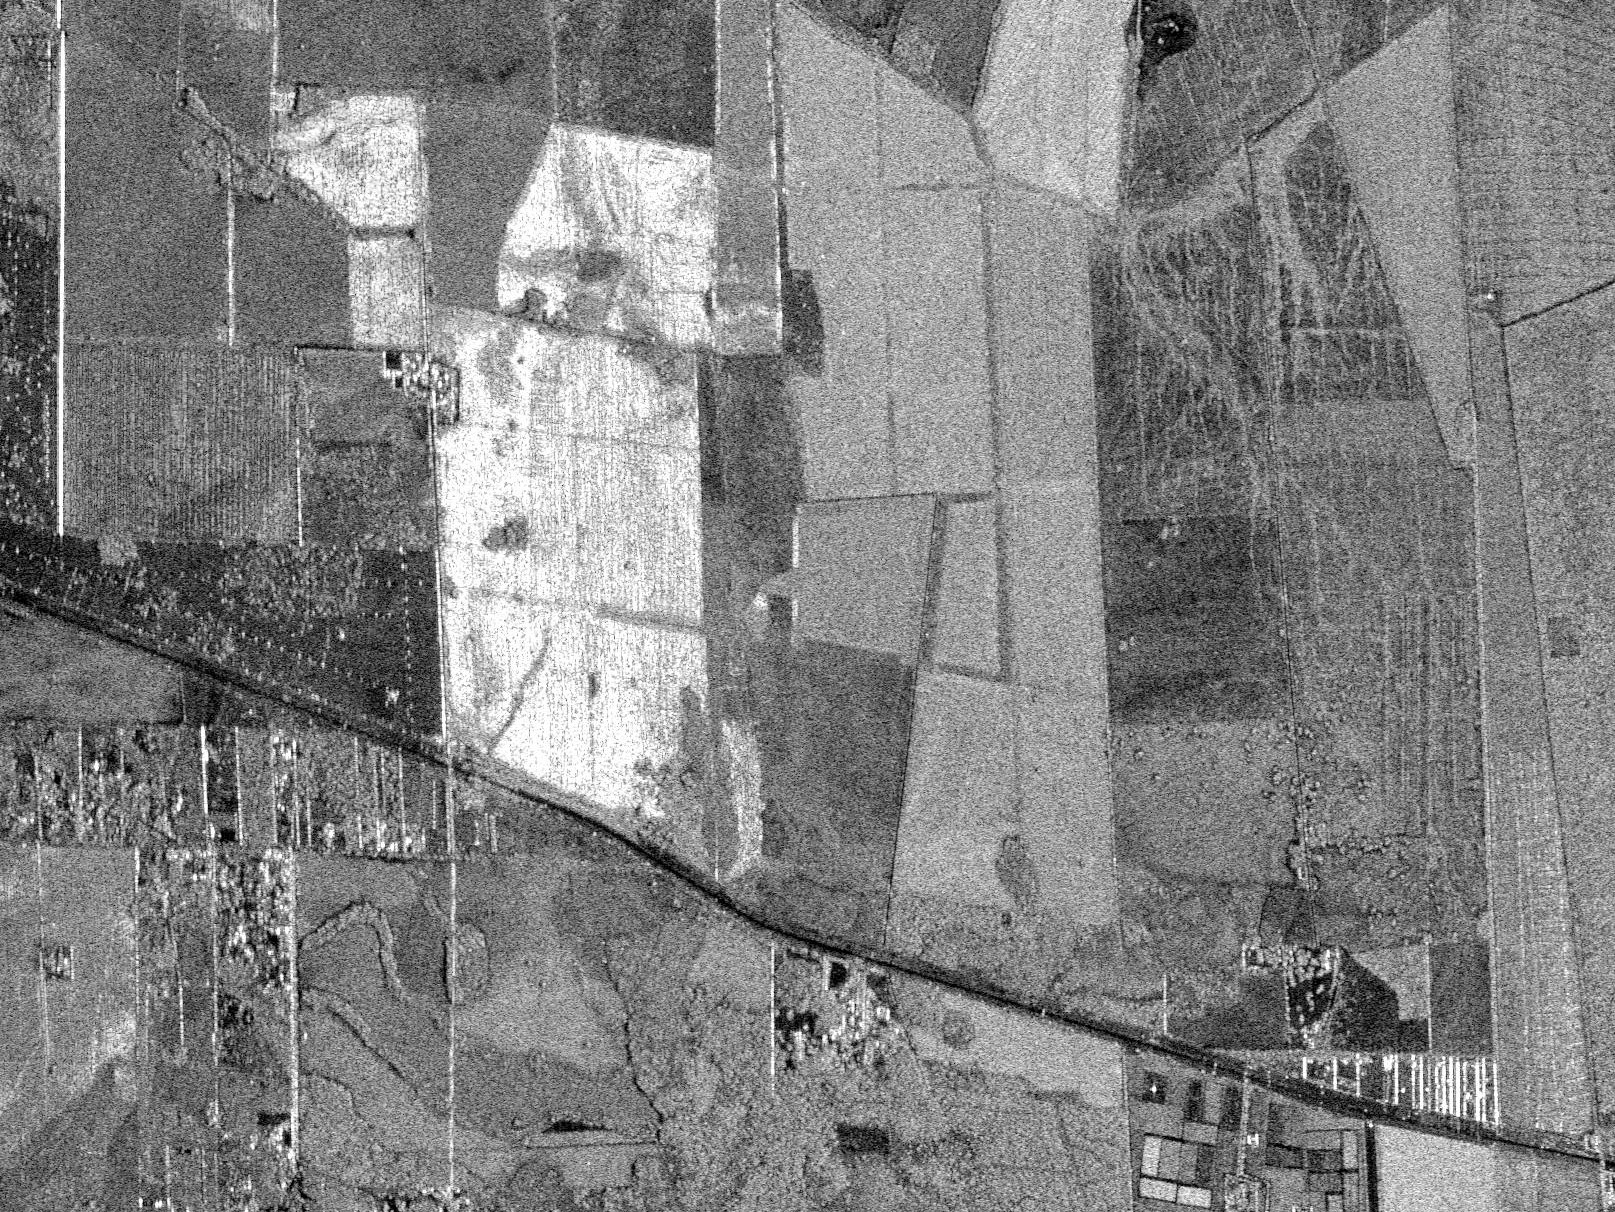
\includegraphics[width=0.25\textwidth]{fig:HH.jpg}}\hspace{1cm}
    \subfloat[Polarización HV]{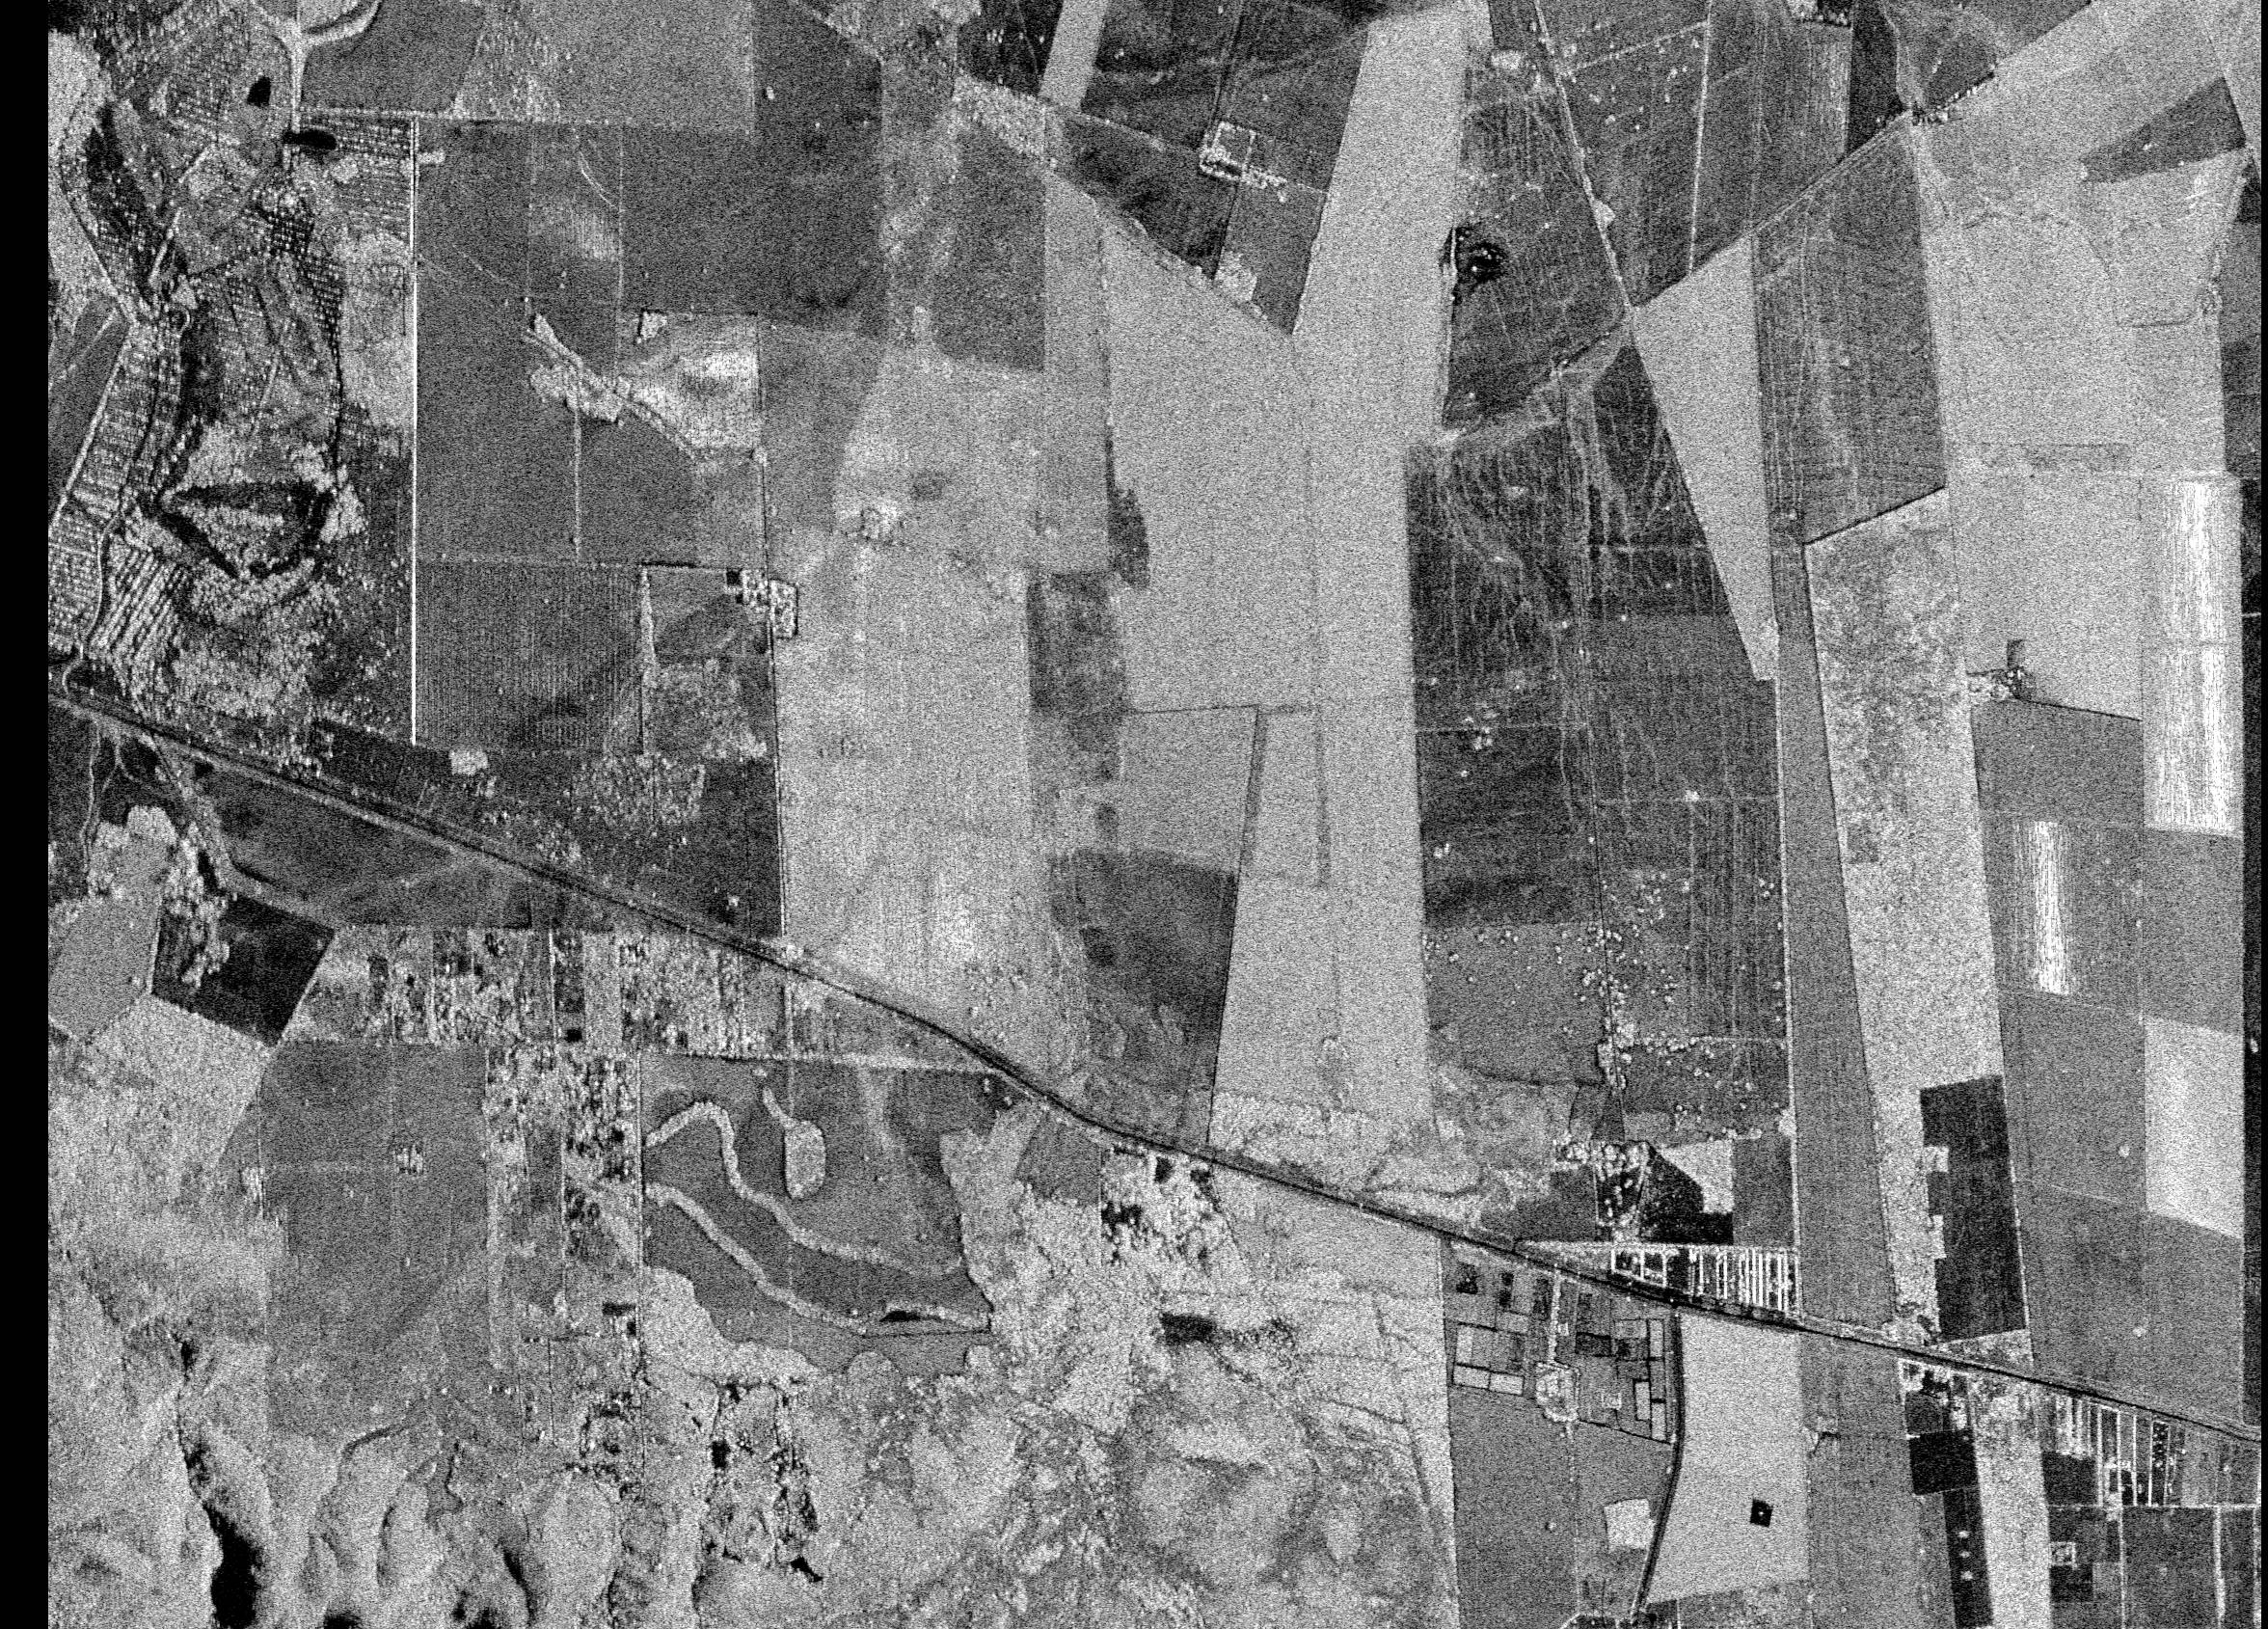
\includegraphics[width=0.25\textwidth]{fig:HV.jpg}}
    \\
    \subfloat[Polarización VH]{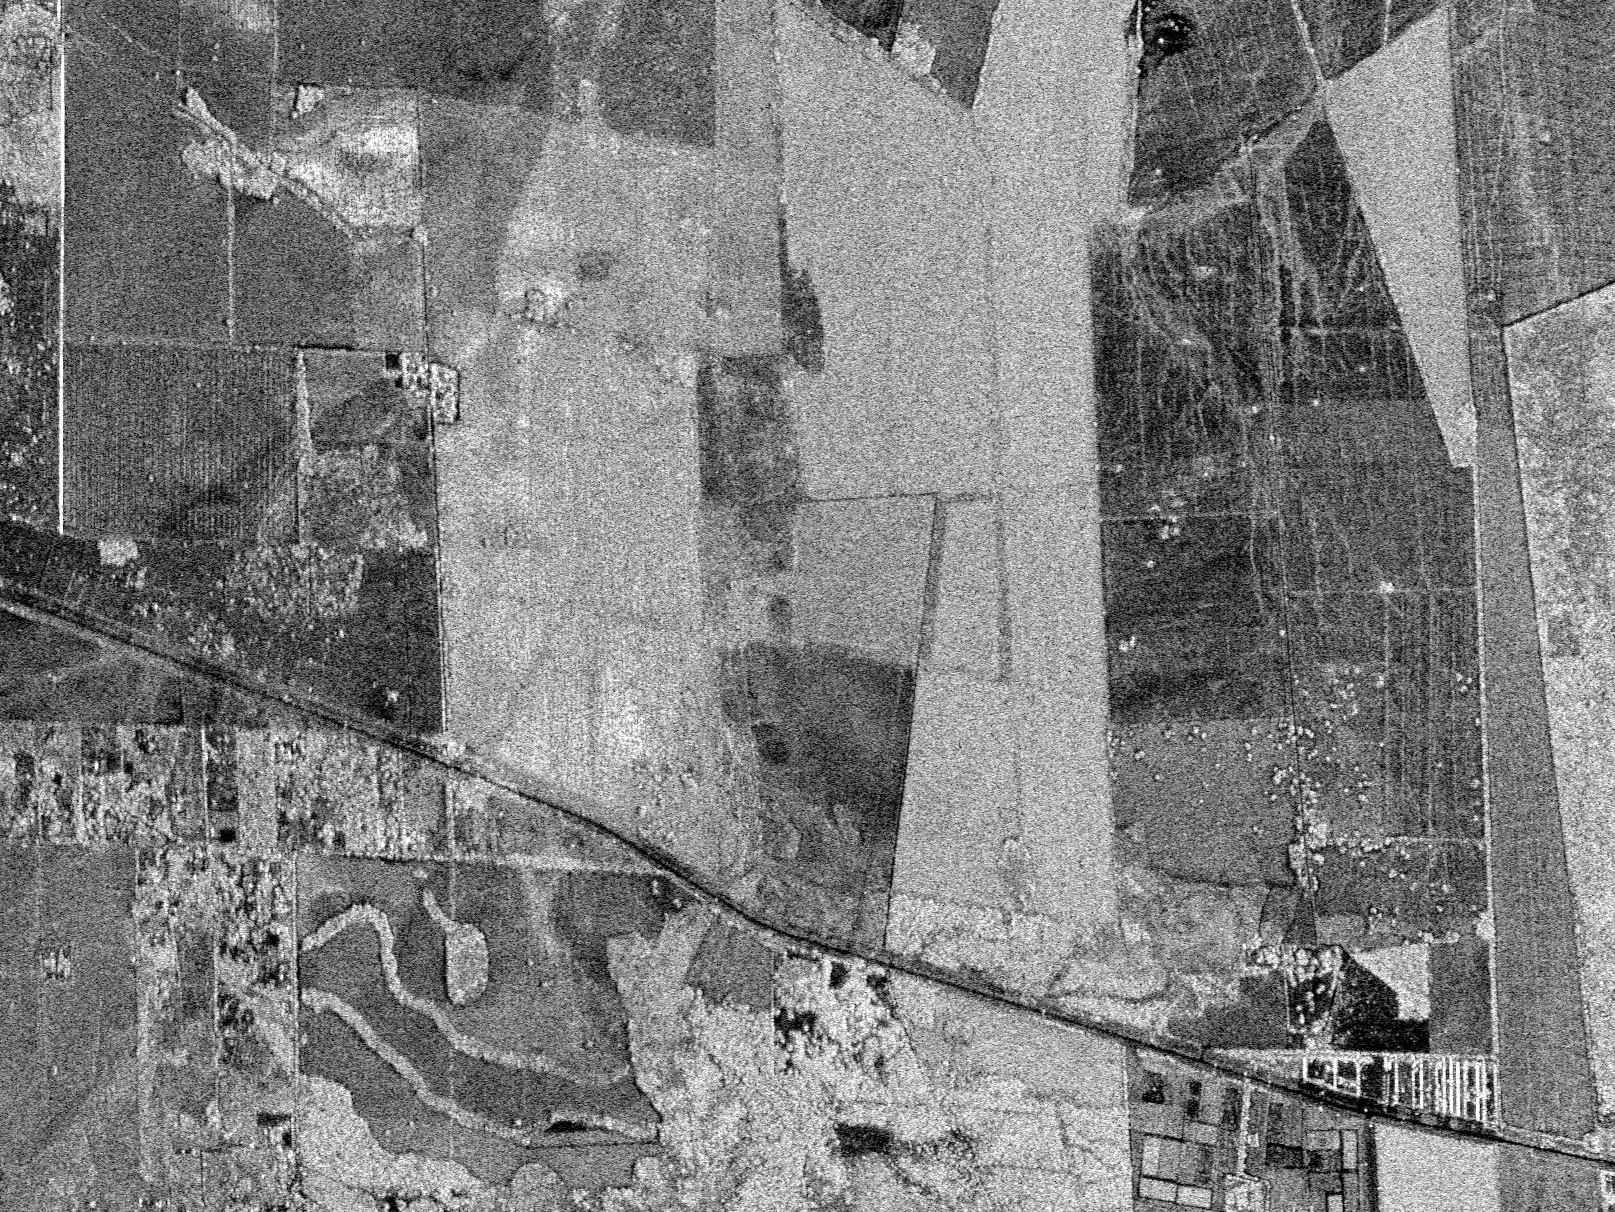
\includegraphics[width=0.25\textwidth]{fig:VH.jpg}}\hspace{1cm}
    \subfloat[Polarización VV]{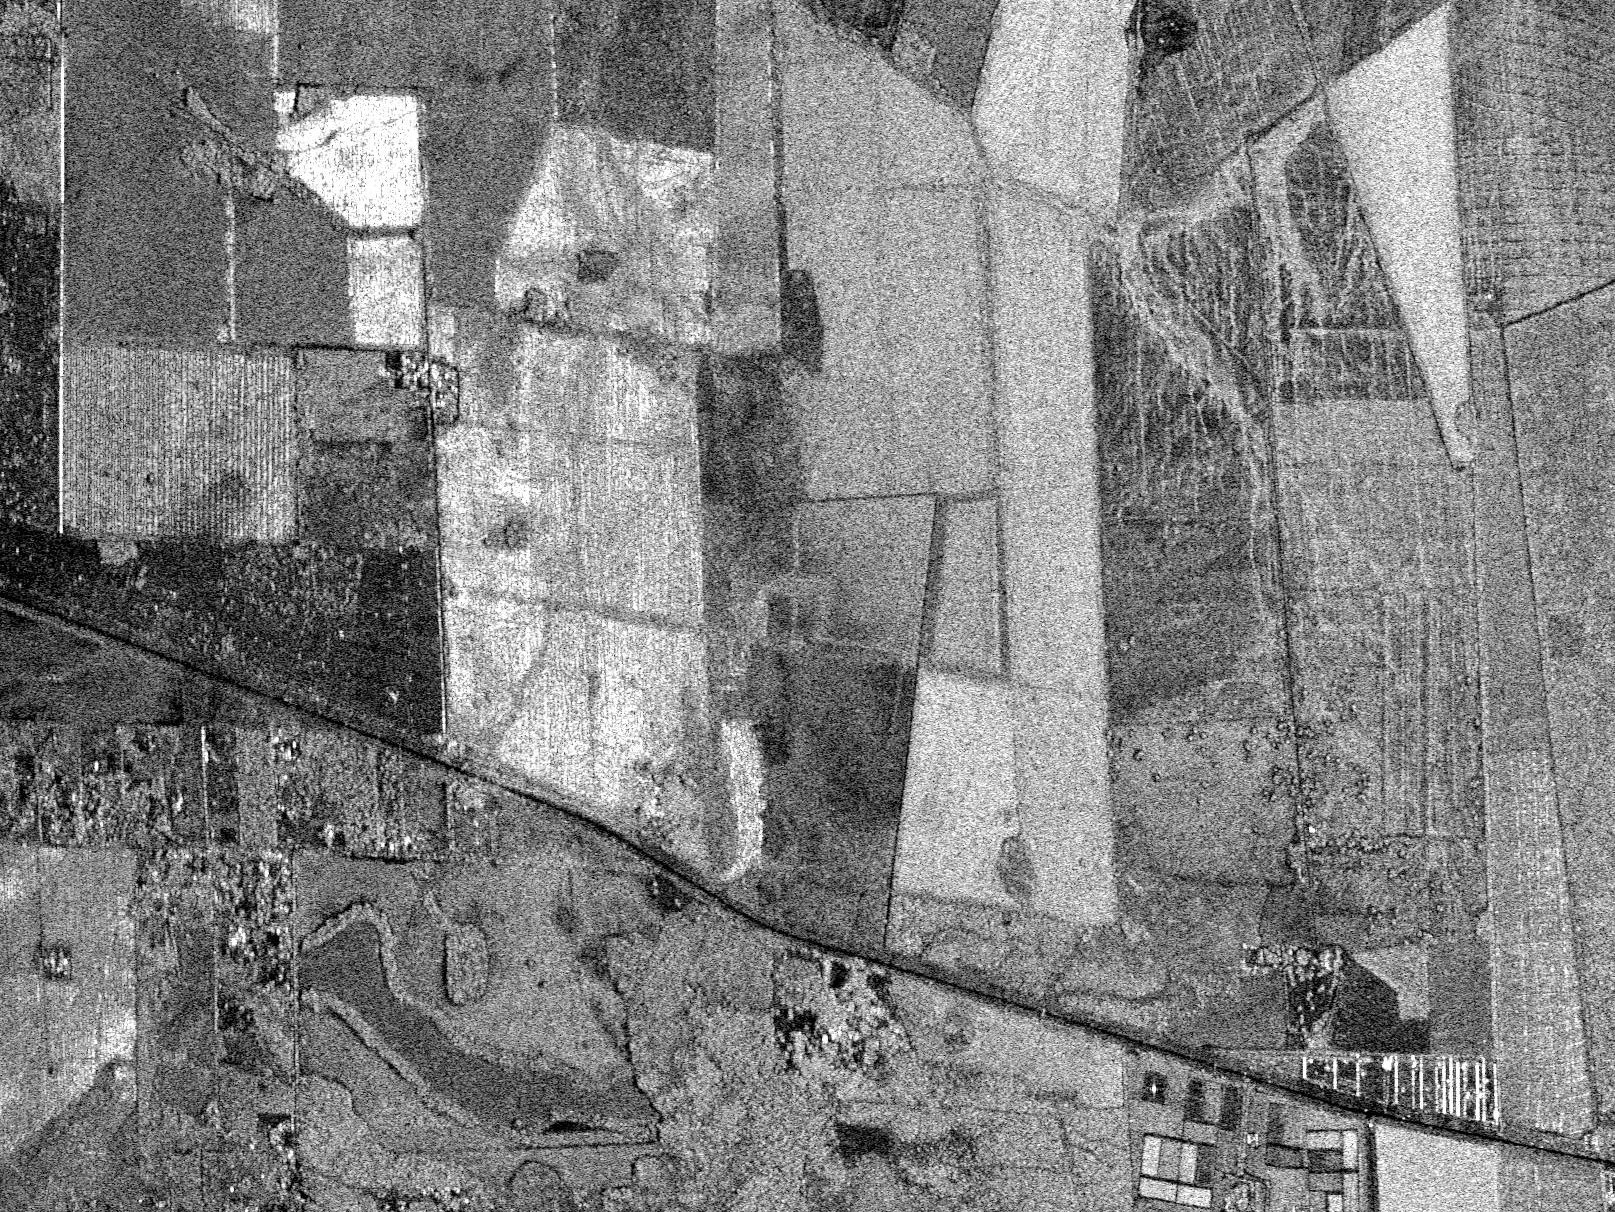
\includegraphics[width=0.25\textwidth]{fig:VV.jpg}}
    \caption{Distintas polarizaciones para una misma región.}
  \end{figure}
\end{frame}
%--- Next Frame ---%

\begin{frame}{\secname : \subsecname}
  En este caso la representación del coeficiente de backscatter es matricial
  \begin{columns}
    \begin{column}{0.5\textwidth}
     \begin{block}{Matriz de scattering}
      \begin{equation}
        S=
  \begin{bmatrix}
    S_{HH} & S_{HV} \\
    S_{VH} & S_{VV}
  \end{bmatrix}
      \end{equation}
     \end{block}
    \end{column}
    \begin{column}{0.5\textwidth}  %%<--- here
      \begin{block}{Matriz de backscatter}
        \begin{equation}
          \sigma_0= \frac{1}{A}
  \begin{bmatrix}
    |S_{HH}|^2 & |S_{HV}|^2 \\
    |S_{VH}|^2 & |S_{VV}|^2
  \end{bmatrix}
        \end{equation}
        con $A$ el area del píxel.
      \end{block}
    \end{column}
    \end{columns}
\end{frame}
%--- Next Frame ---%

\subsection{Descoposición de Pauli}

\begin{frame}{\secname : \subsecname}
     \begin{block}{Descomposición de Paulo}
      \begin{equation}
        R = \left(\frac{HH-VV}{\sqrt{2}}\right)^2
      \end{equation}
      \begin{equation}
        G = \left(\sqrt{2}HV\right)^2
      \end{equation}
      \begin{equation}
        R = \left(\frac{HH+VV}{\sqrt{2}}\right)^2
      \end{equation}
     \end{block}
    La descomposición de Pauli es una manera de visual de ver los distintos mecanismo de scattering presentes: azul -especular-, verde -en volumen- y rojo -doble rebote-.
\end{frame}
%--- Next Frame ---%

\begin{frame}{\secname : \subsecname}
  \begin{figure}
    \centering
    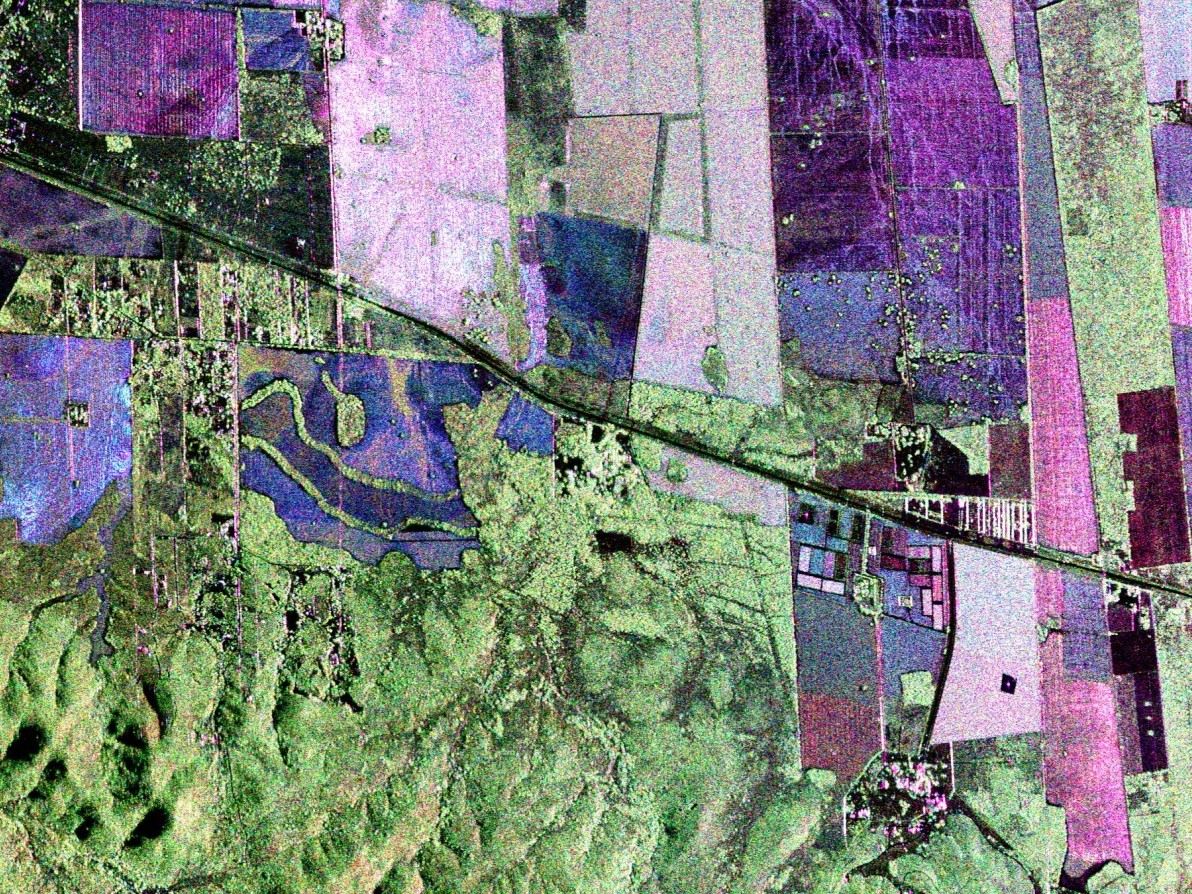
\includegraphics[width=0.5\textwidth]{fig:rgbpauli}
    \caption{Descomposición de Pauli en combinación RGB.}
    \label{}
  \end{figure}
\end{frame}
%--- Next Frame ---%
